\documentclass{report}
\usepackage[spanish]{babel}
\usepackage[left=2.5cm, right=2.5cm, top=3cm, bottom=3cm]{geometry}
\usepackage{enumerate}
\usepackage{geometry}
\usepackage{graphicx}
\usepackage{booktabs}
\usepackage{tabularx}
\usepackage{enumitem}
\usepackage{amsmath}
\usepackage{amsfonts}
\usepackage{float}
\usepackage{hyperref}   

\geometry{
  top=2cm,  bottom=2cm,  left=1.5cm,  right=1.5cm
}

\setlength{\parindent}{0pt}

\begin{document}

    \begin{titlepage}
        \centering
        {\bfseries\LARGE Facultad de Matemática y Computación \par}
        \vspace*{1cm}
        {\scshape\Large Base de Datos II \par}
        \vspace*{3cm}
        {\scshape\Huge Diseño de la base de datos \par}
        \vspace*{1cm}
        {\LARGE \textbf{Tema: Gestión de campeonatos de béisbol} }
        \vfill
        {\bfseries\LARGE Integrantes: \par}
        {\Large Ariadna Vel\'azquez Rey  C311 \par} 
        {\Large L\'ia L\'opez Rosales  C312 \par} 
        {\Large Carlos Daniel Largacha Leal  C312 \par} 
        {\Large Gabriel Andr\'es Pla Lasa  C311 \par} 
        {\Large Raidel Miguel Cabellud Lizaso C311 \par} 
        \vfill
    \end{titlepage}


    \section*{Introducción}

    En este informe se presenta y justifica el diseño de la base de datos a utilizar en el proyecto `` Gestión de 
    campeonatos de béisbol '', para ello se mostrará el Modelo Conceptual (MERX) realizado por el equipo de 
    desarrollo, así como el Modelo Relacional y una justificación del mismo. Además se mencionarán los 
    requerimientos que presenta el proyecto para un mayor entendimiento de la organización de la base de datos.

    \section*{Requerimientos}
    Tras el análisis de la orientación del proyecto y la posterior consulta con algunos de los clientes, se llegó
    a determinar que los requerimientos son:

    \subsection*{Requerimientos Funcionales}
    \begin{enumerate}
        \item Registrar datos por el administrador mediante formularios.
        \item Generar modelos tabulares y gr\'aficos.
        \item Gestionar los roles de la base de datos: usuarios especiales (administrador), los directores técnicos y 
        los usuarios normales (periodistas).
        \item Presentar diferentes vistas para los distintos tipos de roles.
        \item Generar formularios para ingresar los datos a la base de datos por parte del administrador.
        \item Tener un formulario para el director técnico que le permita realizar los cambios en la alineación.
        \item Mostrar un formulario con opciones de filtrado y solicitudes para la generaci\'on de los reportes.
        \item Obtener nombres de equipos ganadores y directores técnicos en series nacionales por temporada.
        \item Obtener nombres y posiciones de jugadores del equipo ``Todos Estrellas'' y su efectividad por serie.
        \item Obtener series con mayor y menor cantidad de juegos celebrados.
        \item Listar equipos en primer y último lugar por serie, clasificados por tipo y orden cronológico.
        \item Obtener el total de juegos ganados por un lanzador y su promedio de carreras limpias permitidas.
        \item Modificar la posición de un jugador en la alineación inicial de un juego específico.
        \item Obtener estadísticas de un jugador.
        \item Exportar reportes a formato PDF, con soporte para la agregación de otros formatos.
    \end{enumerate}

    \subsection*{Requerimientos No Funcionales}

    \subsubsection*{Usabilidad}
    \begin{itemize}
        \item Se espera que la interfaz sea capaz de mostrar gráficas.
        \item Se espera un sistema visual de filtrado para seleccionar qué datos mostrar en los reportes.
    \end{itemize}

    \subsubsection*{Seguridad}
    \begin{itemize}
        \item Todos los datos personales y críticos deben ser encriptados en tránsito y en almacenamiento.
        \item La autenticación y autorización deben ser seguras, permitiendo que solo los usuarios autorizados tengan 
        acceso a funcionalidades específicas.
    \end{itemize}

    \subsubsection*{Portabilidad y Compatibilidad}
    \begin{itemize}
        \item El diseño de la interfaz se espera que sea ajustable al tamaño de los distintos dispositivos en los que 
        puede abrirse el sitio web.
        \item Debe ser compatible con los navegadores más utilizados, asegurando que las interfaces web sean 
        responsivas y adaptativas.
    \end{itemize}

    \subsubsection*{Rendimiento}
    \begin{itemize}
        \item El sistema debe ser capaz de manejar múltiples solicitudes simultáneamente sin una degradación 
        significativa en el tiempo de respuesta.
    \end{itemize}

    \subsubsection*{Escalabilidad}
    \begin{itemize}
        \item La arquitectura debe permitir la escalabilidad horizontal y vertical. Esto significa que se debe poder 
        agregar más recursos (como servidores adicionales) para manejar un mayor número de usuarios o datos sin 
        necesidad de reestructurar significativamente el sistema.
    \end{itemize}

    \subsubsection*{Mantenibilidad}
    \begin{itemize}
        \item El sistema debe estar desarrollado con buenas prácticas de programación, como la documentación adecuada 
        (docstring) y código modular.
    \end{itemize}

    \subsubsection*{Extensibilidad}
    \begin{itemize}
        \item La arquitectura del sistema debe ser flexible para permitir la adición de nuevas funcionalidades sin 
        necesidad de grandes modificaciones en el código base.
    \end{itemize}

    \subsubsection*{Almacenamiento, importación y exportación de datos}
    \begin{itemize}
        \item El software deberá de almacenar todos los datos en una base de datos SQL.
        \item El software deberá ser capaz de convertir los reportes solicitados a documentos PDF.
    \end{itemize}

    \section*{Requerimientos informacionales}

    Para garantizar la consistencia, precisión y confiabilidad de los datos en el sistema de gestión de campeonatos 
    de béisbol, se han definido diversas restricciones de integridad. Estas restricciones aseguran que las 
    relaciones entre peloteros, equipos, series y juegos sean válidas y que los datos almacenados cumplan con las 
    reglas del negocio.

    \subsection*{Datos a almacenar}
    
    A continuación se muestran los datos imprescindibles a almcenar en la base de datos con sus correspondientes entidades.

    \begin{itemize}
        \item \textbf{Usuario:}
        \begin{itemize}
            \item \texttt{email} (\textit{varchar})
        \end{itemize} 

        \item \textbf{Rol:}
        \begin{itemize}
            \item \texttt{tipo} (\textit{varchar})
        \end{itemize}

        \item \textbf{Persona:}
        \begin{itemize}
            \item \texttt{CI} (\textit{integer})
            \item \texttt{Edad} (\textit{integer})
            \item \texttt{NombreP} (\textit{varchar})
            \item \texttt{Apellidos} (\textit{text})
        \end{itemize}

        \item \textbf{Pelotero:}
        \begin{itemize}
            \item \texttt{Años\_de\_experiencia} (\textit{integer}) \newline
        \end{itemize}

        \item \textbf{Equipo:}
        \begin{itemize}
            \item \texttt{Nombre} (\textit{varchar})
            \item \texttt{Color} (\textit{varchar})
            \item \texttt{Iniciales} (\textit{varchar})
            \item \texttt{Entidad\_Representante} (\textit{varchar}) \newline
        \end{itemize}

        \item \textbf{Serie:}
        \begin{itemize}
            \item \texttt{Nombre} (\textit{varchar})
            \item \texttt{Tipo} (\textit{varchar})
            \item \texttt{Fecha\_inicio} (\textit{datetime})
            \item \texttt{Fecha\_fin} (\textit{datetime}) \newline
        \end{itemize}

        \item \textbf{Posición:}
        \begin{itemize}
            \item \texttt{Nombre} (\textit{varchar}) \newline
        \end{itemize}

        \item \textbf{Lanzador:}
        \begin{itemize}
            \item \texttt{Mano\_dominante} (\textit{enum})
            \item \texttt{No\_juegos\_ganados} (\textit{integer})
            \item \texttt{No\_juegos\_perdidos} (\textit{integer}) \newline
        \end{itemize}

        \item \textbf{Jugador en Posición:}
        \begin{itemize}
            \item \texttt{Efectividad} (\textit{double}) \newline
        \end{itemize}

        \item \textbf{Juego:}
        \begin{itemize}
            \item \texttt{Fecha} (\textit{datetime})
            \item \texttt{Equipo ganador} (\textit{integer}) 
            \item \texttt{Equipo perdedor} (\textit{integer})
            \item \texttt{Puntos del ganador} (\textit{integer}) 
            \item \texttt{Puntos del perdedor} (\textit{integer}) \newline
        \end{itemize}

        \item \textbf{Cambio de Jugadores:}
        \begin{itemize}
            \item \texttt{Fecha} (\textit{datetime}) -- Con Hora
            \item \texttt{Jugador (entrante)} (\textit{integer}) 
            \item \texttt{Jugador (saliente)} (\textit{integer}) \newline
        \end{itemize}
            
    \end{itemize}

    \subsection*{Integridad de Dominio y Restriciones de Integridad}
    
    Y luego se muestran la integridad de los datos y un conjunto de restricciones que los datos deben cumplir.

    \begin{itemize}
        \item \textbf{Dominio para fechas:} 
        \begin{align*}
            \texttt{FechaInicio} < \texttt{FechaFin}
        \end{align*}

        \item \textbf{Dominio para estadísticas:} 
        \begin{align*}
            \texttt{JuegosGanados} \geq 0, \hspace*{0.9cm} \texttt{JuegosPerdidos} \geq 0, \hspace*{0.9cm} \texttt{PromedioCarreras} \geq 0
        \end{align*}

        \item \textbf{Dominio para posiciones:} Los valores de las posiciones deben estar restringidos a:
        \begin{align*}
            \{\texttt{pitcher, catcher, baseman, outfielder, shortstop, etc.}\}
        \end{align*}

        \item \textbf{Dominio para atributos específicos:} 
        \begin{align*}
            \texttt{ManoDominante} \in \{\texttt{derecha, izquierda}\}
        \end{align*}

        \item \textbf{Unicidad de pelotero por serie:} Un pelotero no puede pertenecer a más de un equipo dentro de 
        la misma serie.
        \begin{align*}
            \texttt{UNIQUE(Pelotero\_ID, Serie\_ID)}
        \end{align*}

        \item \textbf{Resultados de juegos:} En un juego deben registrarse un equipo ganador y uno perdedor, y no 
        pueden ser el mismo.
        \begin{align*}
            \texttt{Ganador\_ID} \neq \texttt{Perdedor\_ID}
        \end{align*}

        \item \textbf{Alineación única por juego y equipo:} Un jugador no puede estar en más de una posición en la 
        alineación inicial de un equipo durante un juego específico.
        \begin{align*}
            \texttt{UNIQUE(Juego\_ID, Equipo\_ID, Pelotero\_ID)}
        \end{align*}

        \item \textbf{Relación entre estadísticas y jugadores:} Si un jugador es registrado como lanzador, deben incluirse sus estadísticas específicas.
        \begin{align*}
            \texttt{JuegosGanados}, \texttt{JuegosPerdidos}, \texttt{PromedioCarreras}
        \end{align*}

        \item \textbf{Jugador estrella:} Los jugadores estrella deben seleccionarse al final de cada serie y no 
        duplicarse para una misma posición en la misma serie.
    \end{itemize}

    \newpage

    \section*{Modelo Conceptual}

    En la \textit{Figura 1} se encuentra el gráfico del MERX que se utilizará como base en el diseño de la base de 
    datos.

    \begin{figure}[H] 
        \centering
        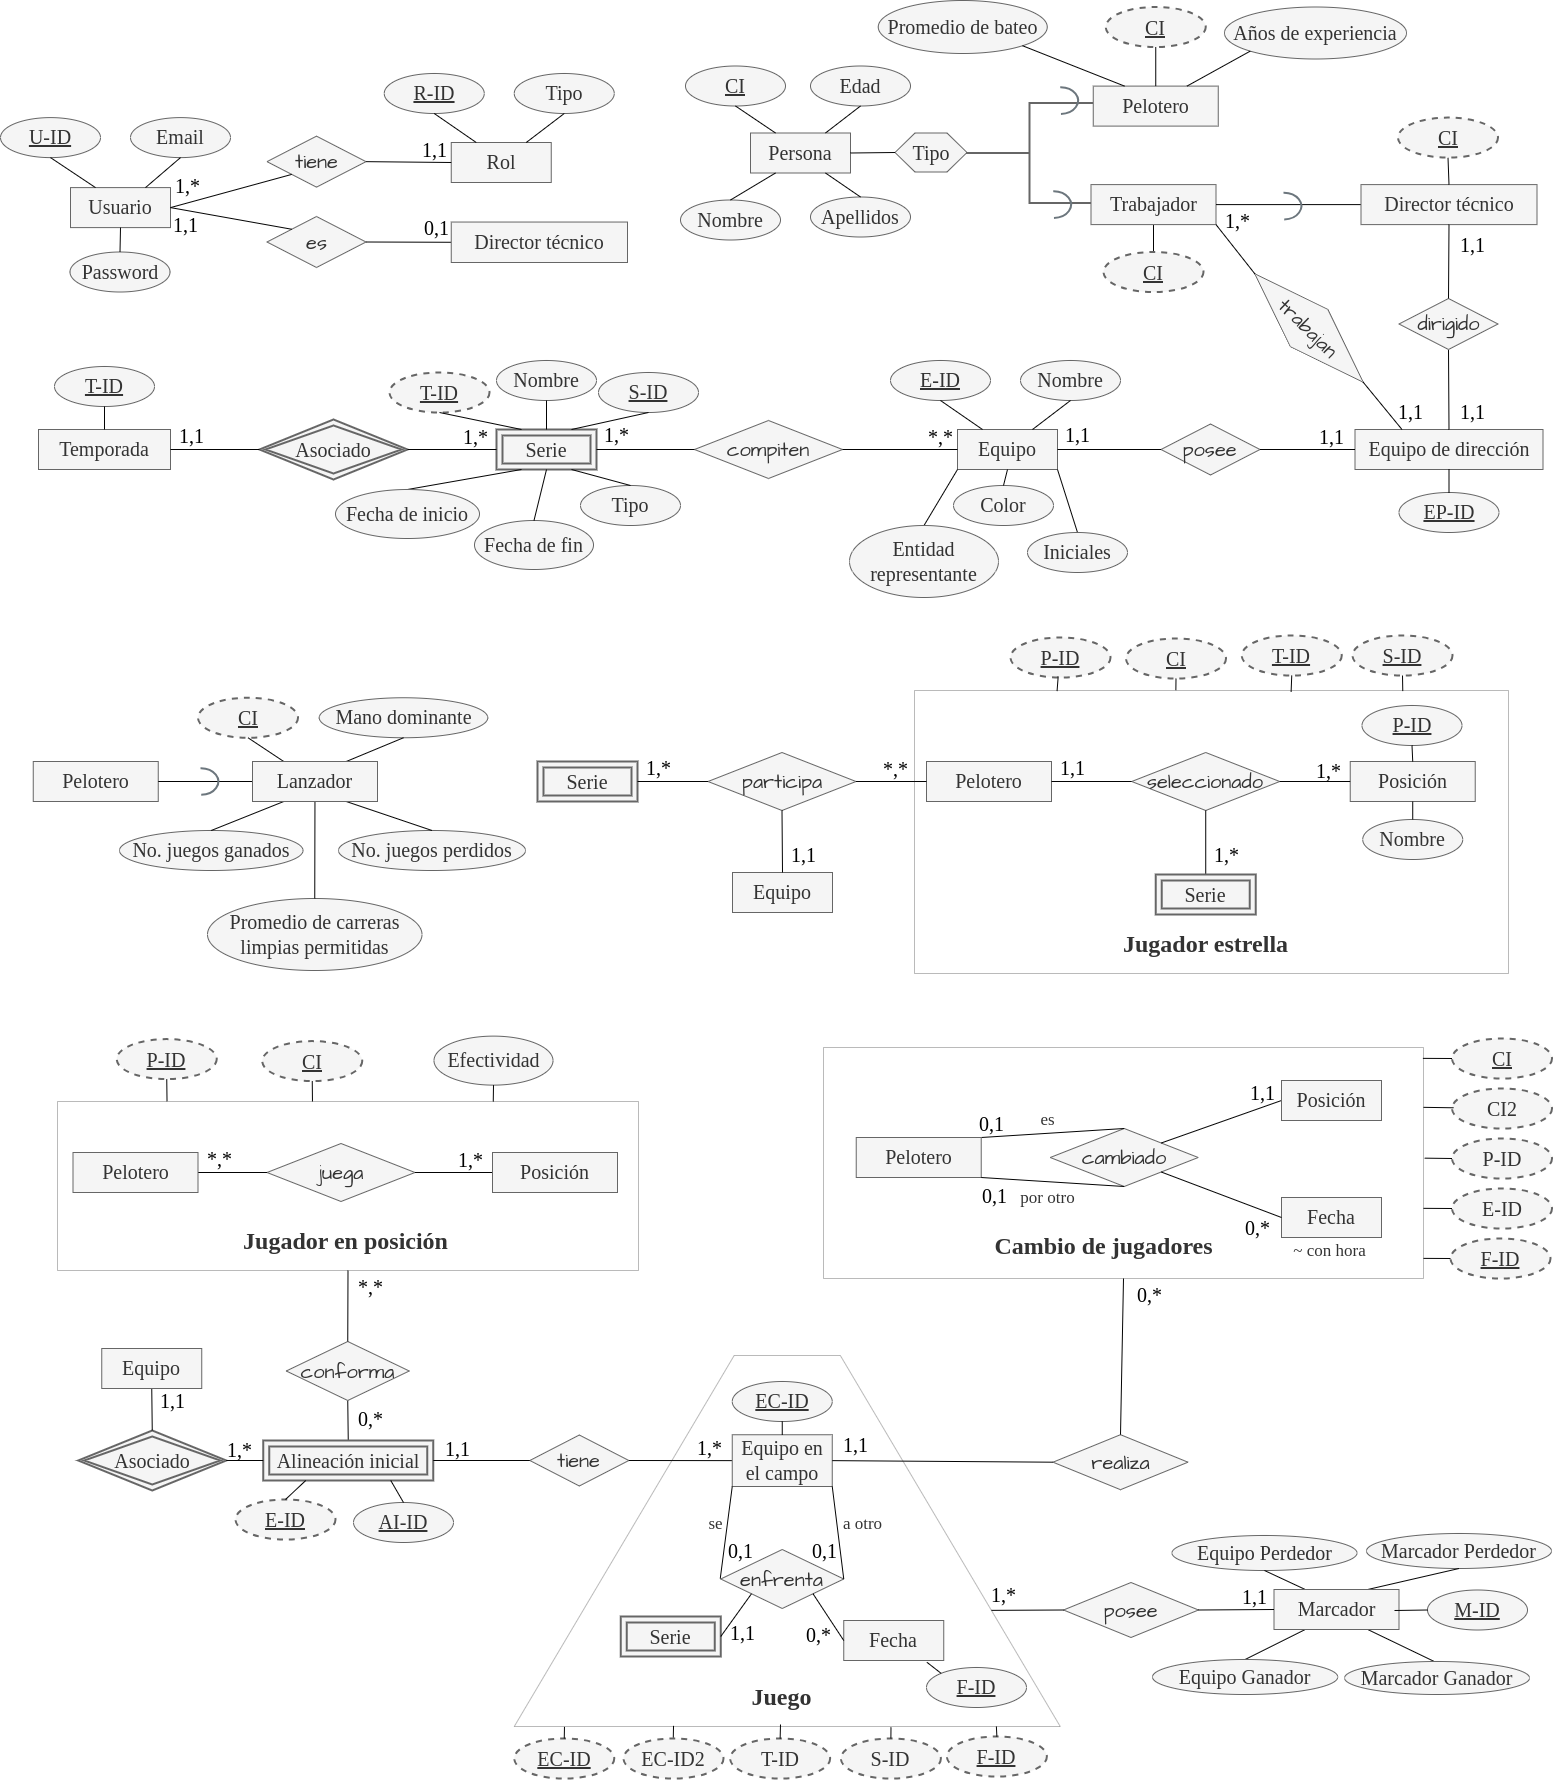
\includegraphics[scale=0.33, keepaspectratio]{baseball_MERX.png}
        \caption{MERX de la Gestión de campeonatos de béisbol}
    \end{figure}

    \newpage

    \section*{Modelo Relacional}

    A partir del MERX propuesto, se identificaron las dependencias funcionales que describen cómo los atributos de cada entidad y sus relaciones están determinados por sus claves primarias.
    En la siguiente tabla se muestran el universo y las dependencias funcionales obtenidas: \newline
    
    \begin{tabularx}{\textwidth}{|X|}
        \toprule
        \hfil $\textbf{R(U, F)}$ \\
        \midrule
        \vspace*{0.01cm}
        $U = \{ $ TipoR, Marcador Ganador, Fecha de fin, No juegos ganados, S-ID, EC-ID, Lanzador, Email, Password, DT-ID, P-ID, F-ID, Apellidos, W-ID, Color, Fecha de inicio, BP-ID, Iniciales, Años de experiencia, R-ID, Edad, TipoS, Promedio de bateo, U-ID, ED-ID, EC-ID 2, Mano dominante, NombreE, NombrePos, No juegos perdidos, M-ID, NombreP, Promedio carreras, BP-ID 2, NombreTS, CI, AI-ID, E-ID, Marcador Perdedor, T-ID, Entidad representante, E-ID 2, Efectividad $\} $ 
        \vspace*{0.15cm} \\
        \midrule
        \vspace*{0.01cm}
        $F = \{$
        U-ID $\rightarrow$ Email, Password \newline
        \hspace*{0.9cm} R-ID $\rightarrow$ TipoR, \newline
        \hspace*{0.9cm} U-ID $\rightarrow$ R-ID, \newline
        \hspace*{0.9cm} CI $\rightarrow$ NombreP, Edad, Apellidos, \newline
        \hspace*{0.9cm} BP-ID $\rightarrow$ CI, \newline
        \hspace*{0.9cm} CI $\rightarrow$ BP-ID, \newline
        \hspace*{0.9cm} BP-ID $\rightarrow$ Promedio de bateo, Años de experiencia, \newline
        \hspace*{0.9cm} W-ID $\rightarrow$ CI, \newline
        \hspace*{0.9cm} CI $\rightarrow$ W-ID, \newline
        \hspace*{0.9cm} W-ID $\rightarrow$ DT-ID, \newline
        \hspace*{0.9cm} DT-ID $\rightarrow$ W-ID, \newline
        \hspace*{0.9cm} ED-ID $\rightarrow$ ED-ID, \newline
        \hspace*{0.9cm} E-ID $\rightarrow$ NombreE, Color, Entidad representante, Iniciales, \newline
        \hspace*{0.9cm} E-ID, AI-ID $\rightarrow$ E-ID, AI-ID, \newline
        \hspace*{0.9cm} T-ID $\rightarrow$ T-ID, \newline
        \hspace*{0.9cm} T-ID, S-ID $\rightarrow$ NombreTS, TipoS, Fecha de inicio, Fecha de fin, \newline
        \hspace*{0.9cm} P-ID $\rightarrow$ NombrePos, \newline
        \hspace*{0.9cm} BP-ID $\rightarrow$ Lanzador, \newline
        \hspace*{0.9cm} Lanzador $\rightarrow$ BP-ID, \newline
        \hspace*{0.9cm} Lanzador $\rightarrow$ Mano dominante, No juegos ganados, No juegos perdidos, Promedio carreras, \newline
        \hspace*{0.9cm} EC-ID $\rightarrow$ EC-ID, \newline
        \hspace*{0.9cm} F-ID $\rightarrow$ F-ID, \newline
        \hspace*{0.9cm} W-ID $\rightarrow$ ED-ID,  \newline
        \hspace*{0.9cm} DT-ID $\rightarrow$ ED-ID, \newline
        \hspace*{0.9cm} ED-ID $\rightarrow$ DT-ID, \newline
        \hspace*{0.9cm} ED-ID $\rightarrow$ E-ID,  \newline
        \hspace*{0.9cm} E-ID $\rightarrow$ ED-ID, \newline
        \hspace*{0.9cm} T-ID, S-ID, E-ID $\rightarrow$ T-ID, S-ID, E-ID , \newline
        \hspace*{0.9cm} T-ID, S-ID, BP-ID $\rightarrow$ E-ID, \newline
        \hspace*{0.9cm} T-ID, S-ID, P-ID $\rightarrow$ BP-ID, \newline
        \hspace*{0.9cm} BP-ID, P-ID $\rightarrow$ Efectividad, \newline
        \hspace*{0.9cm} E-ID, AI-ID, BP-ID, P-ID $\rightarrow$ E-ID, AI-ID, BP-ID, P-ID, \newline
        \hspace*{0.9cm} EC-ID $\rightarrow$ E-ID, AI-ID, \newline
        \hspace*{0.9cm} BP-ID, F-ID $\rightarrow$ BP-ID 2, P-ID, \newline
        \hspace*{0.9cm} BP-ID, F-ID $\rightarrow$ EC-ID, \newline
        \hspace*{0.9cm} EC-ID, F-ID $\rightarrow$ EC-ID 2, T-ID, S-ID, \newline
        \hspace*{0.9cm} EC-ID, F-ID $\rightarrow$ M-ID, \newline
        \hspace*{0.9cm} M-ID $\rightarrow$ E-ID, E-ID 2, Marcador Ganador, Marcador Perdedor        
        $\} $
        \vspace*{0.15cm} \\    
        \bottomrule
    \end{tabularx}

    \vspace*{0.3cm}
    En la siguiente tabla se muestran los resultados de aplicar el algoritmo del cubrimiento mínimo a partir de las dependencias funcionales expuestas. 
    El código del algoritmo se puede encontrar en la página de este proyecto en GitHub. \url{https://github.com/gaboCiber/Baseball-Champions/} 

    \begin{tabularx}{\textwidth}{|X|X|X|}
        \toprule
        \hfil F ' & \hfil F ' '  & \hfil F ' ' '  \\
        \midrule
        U-ID $\rightarrow$ Email \newline 
        U-ID $\rightarrow$ Password \newline 
        R-ID $\rightarrow$ TipoR \newline 
        U-ID $\rightarrow$ R-ID \newline 
        CI $\rightarrow$ NombreP \newline 
        CI $\rightarrow$ Edad \newline 
        CI $\rightarrow$ Apellidos \newline 
        BP-ID $\rightarrow$ CI \newline 
        BP-ID $\rightarrow$ Promedio de bateo \newline 
        BP-ID $\rightarrow$ Años de experiencia \newline 
        W-ID $\rightarrow$ CI \newline 
        W-ID $\rightarrow$ DT-ID \newline 
        DT-ID $\rightarrow$ W-ID \newline 
        E-ID $\rightarrow$ NombreE \newline 
        E-ID $\rightarrow$ Color \newline 
        E-ID $\rightarrow$ Entidad representante \newline 
        E-ID $\rightarrow$ Iniciales \newline 
        T-ID, S-ID $\rightarrow$ NombreTS \newline 
        T-ID, S-ID $\rightarrow$ TipoS \newline 
        T-ID, S-ID $\rightarrow$ Fecha de inicio \newline 
        T-ID, S-ID $\rightarrow$ Fecha de fin \newline 
        P-ID $\rightarrow$ NombrePos \newline 
        BP-ID $\rightarrow$ Lanzador \newline 
        Lanzador $\rightarrow$ BP-ID \newline 
        Lanzador $\rightarrow$ Mano dominante \newline 
        Lanzador $\rightarrow$ No juegos ganados \newline 
        Lanzador $\rightarrow$ No juegos perdidos \newline 
        Lanzador $\rightarrow$ Promedio carreras \newline 
        W-ID $\rightarrow$ ED-ID \newline 
        DT-ID $\rightarrow$ ED-ID \newline 
        ED-ID $\rightarrow$ DT-ID \newline 
        ED-ID $\rightarrow$ E-ID \newline 
        E-ID $\rightarrow$ ED-ID \newline 
        T-ID, S-ID, E-ID $\rightarrow$ T-ID \newline 
        T-ID, S-ID, E-ID $\rightarrow$ S-ID \newline 
        T-ID, S-ID, E-ID $\rightarrow$ E-ID \newline 
        T-ID, S-ID, BP-ID $\rightarrow$ E-ID \newline 
        T-ID, S-ID, P-ID $\rightarrow$ BP-ID \newline 
        BP-ID, P-ID $\rightarrow$ Efectividad \newline 
        E-ID, AI-ID, BP-ID, P-ID $\rightarrow$ E-ID \newline 
        E-ID, AI-ID, BP-ID, P-ID $\rightarrow$ AI-ID \newline 
        E-ID, AI-ID, BP-ID, P-ID $\rightarrow$ BP-ID \newline 
        E-ID, AI-ID, BP-ID, P-ID $\rightarrow$ P-ID \newline 
        EC-ID $\rightarrow$ E-ID \newline 
        EC-ID $\rightarrow$ AI-ID \newline 
        BP-ID, F-ID $\rightarrow$ BP-ID 2 \newline 
        BP-ID, F-ID $\rightarrow$ P-ID \newline 
        BP-ID, F-ID $\rightarrow$ EC-ID \newline 
        EC-ID, F-ID $\rightarrow$ EC-ID 2 \newline 
        EC-ID, F-ID $\rightarrow$ T-ID \newline 
        EC-ID, F-ID $\rightarrow$ S-ID \newline 
        EC-ID, F-ID $\rightarrow$ M-ID \newline 
        M-ID $\rightarrow$ E-ID \newline 
        M-ID $\rightarrow$ E-ID 2 \newline 
        M-ID $\rightarrow$ Marcador Ganador \newline 
        M-ID $\rightarrow$ Marcador Perdedor & 

        U-ID $\rightarrow$ Email \newline 
        U-ID $\rightarrow$ Password \newline 
        R-ID $\rightarrow$ TipoR \newline 
        U-ID $\rightarrow$ R-ID \newline 
        CI $\rightarrow$ NombreP \newline 
        CI $\rightarrow$ Edad \newline 
        CI $\rightarrow$ Apellidos \newline 
        BP-ID $\rightarrow$ CI \newline 
        BP-ID $\rightarrow$ Promedio de bateo \newline 
        BP-ID $\rightarrow$ Años de experiencia \newline 
        W-ID $\rightarrow$ CI \newline 
        W-ID $\rightarrow$ DT-ID \newline 
        DT-ID $\rightarrow$ W-ID \newline 
        E-ID $\rightarrow$ NombreE \newline 
        E-ID $\rightarrow$ Color \newline 
        E-ID $\rightarrow$ Entidad representante \newline 
        E-ID $\rightarrow$ Iniciales \newline 
        T-ID, S-ID $\rightarrow$ NombreTS \newline 
        T-ID, S-ID $\rightarrow$ TipoS \newline 
        T-ID, S-ID $\rightarrow$ Fecha de inicio \newline 
        T-ID, S-ID $\rightarrow$ Fecha de fin \newline 
        P-ID $\rightarrow$ NombrePos \newline 
        BP-ID $\rightarrow$ Lanzador \newline 
        Lanzador $\rightarrow$ BP-ID \newline 
        Lanzador $\rightarrow$ Mano dominante \newline 
        Lanzador $\rightarrow$ No juegos ganados \newline 
        Lanzador $\rightarrow$ No juegos perdidos \newline 
        Lanzador $\rightarrow$ Promedio carreras \newline 
        W-ID $\rightarrow$ ED-ID \newline 
        DT-ID $\rightarrow$ ED-ID \newline 
        ED-ID $\rightarrow$ DT-ID \newline 
        ED-ID $\rightarrow$ E-ID \newline 
        E-ID $\rightarrow$ ED-ID \newline 
        T-ID, S-ID, BP-ID $\rightarrow$ E-ID \newline 
        T-ID, S-ID, P-ID $\rightarrow$ BP-ID \newline 
        BP-ID, P-ID $\rightarrow$ Efectividad \newline 
        EC-ID $\rightarrow$ E-ID \newline 
        EC-ID $\rightarrow$ AI-ID \newline 
        BP-ID, F-ID $\rightarrow$ BP-ID 2 \newline 
        BP-ID, F-ID $\rightarrow$ P-ID \newline 
        BP-ID, F-ID $\rightarrow$ EC-ID \newline 
        EC-ID, F-ID $\rightarrow$ EC-ID 2 \newline 
        EC-ID, F-ID $\rightarrow$ T-ID \newline 
        EC-ID, F-ID $\rightarrow$ S-ID \newline 
        EC-ID, F-ID $\rightarrow$ M-ID \newline 
        M-ID $\rightarrow$ E-ID \newline 
        M-ID $\rightarrow$ E-ID 2 \newline 
        M-ID $\rightarrow$ Marcador Ganador \newline 
        M-ID $\rightarrow$ Marcador Perdedor & 

        U-ID $\rightarrow$ Email \newline 
        U-ID $\rightarrow$ Password \newline 
        R-ID $\rightarrow$ TipoR \newline 
        U-ID $\rightarrow$ R-ID \newline 
        CI $\rightarrow$ NombreP \newline 
        CI $\rightarrow$ Edad \newline 
        CI $\rightarrow$ Apellidos \newline 
        BP-ID $\rightarrow$ CI \newline 
        BP-ID $\rightarrow$ Promedio de bateo \newline 
        BP-ID $\rightarrow$ Años de experiencia \newline 
        W-ID $\rightarrow$ CI \newline 
        DT-ID $\rightarrow$ W-ID \newline 
        E-ID $\rightarrow$ NombreE \newline 
        E-ID $\rightarrow$ Color \newline 
        E-ID $\rightarrow$ Entidad representante \newline 
        E-ID $\rightarrow$ Iniciales \newline 
        T-ID, S-ID $\rightarrow$ NombreTS \newline 
        T-ID, S-ID $\rightarrow$ TipoS \newline 
        T-ID, S-ID $\rightarrow$ Fecha de inicio \newline 
        T-ID, S-ID $\rightarrow$ Fecha de fin \newline 
        P-ID $\rightarrow$ NombrePos \newline 
        BP-ID $\rightarrow$ Lanzador \newline 
        Lanzador $\rightarrow$ BP-ID \newline 
        Lanzador $\rightarrow$ Mano dominante \newline 
        Lanzador $\rightarrow$ No juegos ganados \newline 
        Lanzador $\rightarrow$ No juegos perdidos \newline 
        Lanzador $\rightarrow$ Promedio carreras \newline 
        W-ID $\rightarrow$ ED-ID \newline 
        ED-ID $\rightarrow$ DT-ID \newline 
        ED-ID $\rightarrow$ E-ID \newline 
        E-ID $\rightarrow$ ED-ID \newline 
        T-ID, S-ID, BP-ID $\rightarrow$ E-ID \newline 
        T-ID, S-ID, P-ID $\rightarrow$ BP-ID \newline 
        BP-ID, P-ID $\rightarrow$ Efectividad \newline 
        EC-ID $\rightarrow$ E-ID \newline 
        EC-ID $\rightarrow$ AI-ID \newline 
        BP-ID, F-ID $\rightarrow$ BP-ID 2 \newline 
        BP-ID, F-ID $\rightarrow$ P-ID \newline 
        BP-ID, F-ID $\rightarrow$ EC-ID \newline 
        EC-ID, F-ID $\rightarrow$ EC-ID 2 \newline 
        EC-ID, F-ID $\rightarrow$ T-ID \newline 
        EC-ID, F-ID $\rightarrow$ S-ID \newline 
        EC-ID, F-ID $\rightarrow$ M-ID \newline 
        M-ID $\rightarrow$ E-ID \newline 
        M-ID $\rightarrow$ E-ID 2 \newline 
        M-ID $\rightarrow$ Marcador Ganador \newline 
        M-ID $\rightarrow$ Marcador Perdedor  \\
        \bottomrule
    \end{tabularx}

    \newpage

    Luego a partir de la ejecución del algoritmo de cubrimiento mínimo se pudieron identificar los siguientes atributos y dependencias redundantes. \newline

    \textbf{Atributos redundantes:}
    \begin{itemize}
        \item E-ID,  AI-ID $\rightarrow$ E-ID
        \item E-ID,  AI-ID $\rightarrow$ AI-ID
        \item T-ID,  S-ID,  E-ID $\rightarrow$ T-ID
        \item T-ID,  S-ID,  E-ID $\rightarrow$ S-ID
        \item T-ID,  S-ID,  E-ID $\rightarrow$ E-ID
        \item E-ID,  AI-ID,  BP-ID,  P-ID $\rightarrow$ E-ID
        \item E-ID,  AI-ID,  BP-ID,  P-ID $\rightarrow$ AI-ID
        \item E-ID,  AI-ID,  BP-ID,  P-ID $\rightarrow$ BP-ID
        \item E-ID,  AI-ID,  BP-ID,  P-ID $\rightarrow$ P-ID
    \end{itemize}
   
    \textbf{Dependencias redundantes:}
    \begin{itemize}
        \item W-ID $\rightarrow$ DT-ID
        \begin{itemize}
            \item W-ID $\rightarrow$ EP-ID $\land$  EP-ID  $\rightarrow$ DT-ID $\models$ W-ID $\rightarrow$ DT-ID \newline
        \end{itemize}
        
        \item DT-ID $\rightarrow$ EP-ID
        \begin{itemize}
            \item DT-ID $\rightarrow$ W-ID $\land$  W-ID $\rightarrow$ EP-ID $\models$ DT-ID $\rightarrow$ EP-ID  \newline
        \end{itemize}
    \end{itemize}

    Y por lo tanto a partir de lo anteriormente visto se pudo obtener el siguiente conjunto de dependencias funcionales irreducibles. \newline

    \begin{tabularx}{\textwidth}{|X|}
        \toprule
        \hfil \textbf{Cubrimiento mínimo de F(U,R)} \\
        \midrule
        U-ID $\rightarrow$ Email, Password, R-ID \newline 
        R-ID $\rightarrow$ TipoR \newline 
        CI $\rightarrow$ NombreP, Edad, Apellidos \newline 
        BP-ID $\rightarrow$ CI, Promedio de bateo, Años de experiencia, Lanzador \newline 
        W-ID $\rightarrow$ CI, ED-ID \newline 
        DT-ID $\rightarrow$ W-ID \newline 
        E-ID $\rightarrow$ NombreE, Color, Entidad representante, Iniciales, ED-ID \newline 
        T-ID, S-ID $\rightarrow$ NombreTS, TipoS, Fecha de inicio, Fecha de fin \newline 
        P-ID $\rightarrow$ NombrePos \newline 
        Lanzador $\rightarrow$ BP-ID, Mano dominante, No juegos ganados, No juegos perdidos, Promedio carreras \newline 
        ED-ID $\rightarrow$ DT-ID, E-ID \newline 
        BP-ID, T-ID, S-ID $\rightarrow$ E-ID \newline 
        T-ID, S-ID, P-ID $\rightarrow$ BP-ID \newline 
        BP-ID, P-ID $\rightarrow$ Efectividad \newline 
        EC-ID $\rightarrow$ E-ID, AI-ID \newline 
        F-ID, BP-ID $\rightarrow$ BP-ID 2, P-ID, EC-ID \newline 
        EC-ID, F-ID $\rightarrow$ EC-ID 2, T-ID, S-ID, M-ID \newline 
        M-ID $\rightarrow$ E-ID, E-ID 2, Marcador Ganador, Marcador Perdedor \newline 
        AI-ID, E-ID, BP-ID, P-ID $\rightarrow$ AI-ID, E-ID, BP-ID, P-ID \newline \\ 
        \bottomrule
    \end{tabularx}

    \newpage 

    Y entonces una de las posibles llaves cándidatas de este cojunto irreducible de dependencias funcionales es: U-ID, F-ID, BP-ID. \newline

    Esto se debe a que: tanto U-ID como F-ID son atributos que deben pertenecer a toda llave candidata, puesto que,
    no aparecen en la parte derecha de ninguna dependencias funcional del conjunto, es decir, no existe ningún
    otro atributo simple o compuesto que pueda obtener a U-ID o F-ID. \newline
    
    Y por otra parte se tiene que la clausura $\{$BP-ID$\}_{F}^{+}$ = $\mathsf{U} - \{$ U-ID, F-ID$\}$. Por lo tanto U-ID, F-ID, BP-ID es una llave candidata. \newline

    Luego para garantizar un diseño lógico robusto y evitar redundancias, es necesario obtener un esquema de descomposición en Tercera Forma Normal (3FN),
    el cual puede ser obtenido, a partir de de su algoritmo homólogo y tiene como entrada el conjunto irreducible de dependencias funcionales anteriomente expuesto. \newline
      
    \begin{tabularx}{\textwidth}{|X|}
        \toprule
        \hfil \textbf{Descomposición en Tercera Forma Normal (3FN)} \\
        \midrule
        $ R_{1} ( U_{1} , F_{1} ) $ \newline 
        $ U_{1} = \{{Email, \hspace{0.2cm}  Password, \hspace{0.2cm}  R-ID, \hspace{0.2cm}  U-ID}\} $ \newline 
        $ F_{1} = \sqcap_{U_{_{1}}}(F) \equiv \{U-ID \rightarrow Email, \hspace{0.2cm} Password, \hspace{0.2cm} R-ID \} $\newline 
        
        $ R_{2} ( U_{2} , F_{2} ) $ \newline 
        $ U_{2} = \{{R-ID, \hspace{0.2cm}  TipoR}\} $ \newline 
        $ F_{2} = \sqcap_{U_{_{2}}}(F) \equiv \{R-ID \rightarrow TipoR \} $\newline 
        
        $ R_{3} ( U_{3} , F_{3} ) $ \newline 
        $ U_{3} = \{{NombreP, \hspace{0.2cm}  Apellidos, \hspace{0.2cm}  Edad, \hspace{0.2cm}  CI}\} $ \newline 
        $ F_{3} = \sqcap_{U_{_{3}}}(F) \equiv \{CI \rightarrow NombreP, \hspace{0.2cm} Edad, \hspace{0.2cm} Apellidos \} $\newline 
        
        $ R_{4} ( U_{4} , F_{4} ) $ \newline 
        $ U_{4} = \{{A\tilde{n}os \hspace{0.2cm} de \hspace{0.2cm} experiencia, \hspace{0.2cm}  BP-ID, \hspace{0.2cm}  Lanzador, \hspace{0.2cm}  Promedio \hspace{0.2cm} de \hspace{0.2cm} bateo, \hspace{0.2cm}  CI}\} $ \newline 
        $ F_{4} = \sqcap_{U_{_{4}}}(F) \equiv \{BP-ID \rightarrow CI, \hspace{0.2cm} Promedio \hspace{0.2cm} de \hspace{0.2cm} bateo, \hspace{0.2cm} A\tilde{n}os \hspace{0.2cm} de \hspace{0.2cm} experiencia, \hspace{0.2cm} Lanzador \} $\newline 
        
        $ R_{5} ( U_{5} , F_{5} ) $ \newline 
        $ U_{5} = \{{W-ID, \hspace{0.2cm}  ED-ID, \hspace{0.2cm}  CI}\} $ \newline 
        $ F_{5} = \sqcap_{U_{_{5}}}(F) \equiv \{W-ID \rightarrow CI, \hspace{0.2cm} ED-ID \} $\newline 
        
        $ R_{6} ( U_{6} , F_{6} ) $ \newline 
        $ U_{6} = \{{W-ID, \hspace{0.2cm}  DT-ID}\} $ \newline 
        $ F_{6} = \sqcap_{U_{_{6}}}(F) \equiv \{DT-ID \rightarrow W-ID \} $\newline 
        
        $ R_{7} ( U_{7} , F_{7} ) $ \newline 
        $ U_{7} = \{{NombreE, \hspace{0.2cm}  E-ID, \hspace{0.2cm}  Iniciales, \hspace{0.2cm}  Entidad \hspace{0.2cm} representante, \hspace{0.2cm}  ED-ID, \hspace{0.2cm}  Color}\} $ \newline 
        $ F_{7} = \sqcap_{U_{_{7}}}(F) \equiv \{E-ID \rightarrow NombreE, \hspace{0.2cm} Color, \hspace{0.2cm} Entidad \hspace{0.2cm} representante, \hspace{0.2cm} Iniciales, \hspace{0.2cm} ED-ID \} $\newline 
        
        $ R_{8} ( U_{8} , F_{8} ) $ \newline 
        $ U_{8} = \{{NombreTS, \hspace{0.2cm}  S-ID, \hspace{0.2cm}  Fecha \hspace{0.2cm} de \hspace{0.2cm} inicio, \hspace{0.2cm}  Fecha \hspace{0.2cm} de \hspace{0.2cm} fin, \hspace{0.2cm}  T-ID, \hspace{0.2cm}  TipoS}\} $ \newline 
        $ F_{8} = \sqcap_{U_{_{8}}}(F) \equiv \{T-ID, \hspace{0.2cm} S-ID \rightarrow NombreTS, \hspace{0.2cm} TipoS, \hspace{0.2cm} Fecha \hspace{0.2cm} de \hspace{0.2cm} inicio, \hspace{0.2cm} Fecha \hspace{0.2cm} de \hspace{0.2cm} fin \} $\newline 
        
        $ R_{9} ( U_{9} , F_{9} ) $ \newline 
        $ U_{9} = \{{P-ID, \hspace{0.2cm}  NombrePos}\} $ \newline 
        $ F_{9} = \sqcap_{U_{_{9}}}(F) \equiv \{P-ID \rightarrow NombrePos \} $\newline 
        
        $ R_{10} ( U_{10} , F_{10} ) $ \newline 
        $ U_{10} = \{{BP-ID, \hspace{0.2cm}  Promedio \hspace{0.2cm} carreras, \hspace{0.2cm}  Mano \hspace{0.2cm} dominante, \hspace{0.2cm} Juegos \hspace{0.2cm} perdidos, \hspace{0.2cm}  Lanzador, \hspace{0.2cm} Juegos \hspace{0.2cm} ganados}\} $ \newline 
        $ F_{10} = \sqcap_{U_{_{10}}}(F) \equiv \{Lanzador \rightarrow BP-ID, \hspace{0.1cm} Mano \hspace{0.1cm} dominante, \hspace{0.1cm} Juegos \hspace{0.1cm} ganados, \hspace{0.1cm} Juegos \hspace{0.1cm} perdidos, \hspace{0.1cm} Promedio \hspace{0.1cm} carreras \} $\newline \\
        
        \bottomrule
    \end{tabularx}

    \begin{tabularx}{\textwidth}{|X|}
        \toprule
        \hfil \textbf{Descomposición en Tercera Forma Normal (3FN)} \\
        \midrule
        $ R_{11} ( U_{11} , F_{11} ) $ \newline 
        $ U_{11} = \{{E-ID, \hspace{0.2cm}  DT-ID, \hspace{0.2cm}  ED-ID}\} $ \newline 
        $ F_{11} = \sqcap_{U_{_{11}}}(F) \equiv \{ED-ID \rightarrow DT-ID, \hspace{0.2cm} E-ID \} $\newline 
        
        $ R_{12} ( U_{12} , F_{12} ) $ \newline 
        $ U_{12} = \{{BP-ID, \hspace{0.2cm}  T-ID, \hspace{0.2cm}  S-ID, \hspace{0.2cm}  E-ID}\} $ \newline 
        $ F_{12} = \sqcap_{U_{_{12}}}(F) \equiv \{BP-ID, \hspace{0.2cm} T-ID, \hspace{0.2cm} S-ID \rightarrow E-ID \} $\newline 
        
        $ R_{13} ( U_{13} , F_{13} ) $ \newline 
        $ U_{13} = \{{BP-ID, \hspace{0.2cm}  T-ID, \hspace{0.2cm}  S-ID, \hspace{0.2cm}  P-ID}\} $ \newline 
        $ F_{13} = \sqcap_{U_{_{13}}}(F) \equiv \{T-ID, \hspace{0.2cm} S-ID, \hspace{0.2cm} P-ID \rightarrow BP-ID \} $\newline 
        
        $ R_{14} ( U_{14} , F_{14} ) $ \newline 
        $ U_{14} = \{{Efectividad, \hspace{0.2cm}  BP-ID, \hspace{0.2cm}  P-ID}\} $ \newline 
        $ F_{14} = \sqcap_{U_{_{14}}}(F) \equiv \{BP-ID, \hspace{0.2cm} P-ID \rightarrow Efectividad \} $\newline 
        
        $ R_{15} ( U_{15} , F_{15} ) $ \newline 
        $ U_{15} = \{{EC-ID, \hspace{0.2cm}  AI-ID, \hspace{0.2cm}  E-ID}\} $ \newline 
        $ F_{15} = \sqcap_{U_{_{15}}}(F) \equiv \{EC-ID \rightarrow E-ID, \hspace{0.2cm} AI-ID \} $\newline 
        
        $ R_{16} ( U_{16} , F_{16} ) $ \newline 
        $ U_{16} = \{{BP-ID \hspace{0.2cm} 2, \hspace{0.2cm}  BP-ID, \hspace{0.2cm}  EC-ID, \hspace{0.2cm}  F-ID, \hspace{0.2cm}  P-ID}\} $ \newline 
        $ F_{16} = \sqcap_{U_{_{16}}}(F) \equiv \{F-ID, \hspace{0.2cm} BP-ID \rightarrow BP-ID \hspace{0.2cm} 2, \hspace{0.2cm} P-ID, \hspace{0.2cm} EC-ID \} $\newline 
        
        $ R_{17} ( U_{17} , F_{17} ) $ \newline 
        $ U_{17} = \{{EC-ID \hspace{0.2cm} 2, \hspace{0.2cm}  S-ID, \hspace{0.2cm}  M-ID, \hspace{0.2cm}  EC-ID, \hspace{0.2cm}  F-ID, \hspace{0.2cm}  T-ID}\} $ \newline 
        $ F_{17} = \sqcap_{U_{_{17}}}(F) \equiv \{EC-ID, \hspace{0.2cm} F-ID \rightarrow EC-ID \hspace{0.2cm} 2, \hspace{0.2cm} T-ID, \hspace{0.2cm} S-ID, \hspace{0.2cm} M-ID \} $\newline 
        
        $ R_{18} ( U_{18} , F_{18} ) $ \newline 
        $ U_{18} = \{{E-ID \hspace{0.2cm} 2, \hspace{0.2cm}  E-ID, \hspace{0.2cm}  M-ID, \hspace{0.2cm}  Marcador \hspace{0.2cm} Ganador, \hspace{0.2cm}  Marcador \hspace{0.2cm} Perdedor}\} $ \newline 
        $ F_{18} = \sqcap_{U_{_{18}}}(F) \equiv \{M-ID \rightarrow E-ID, \hspace{0.2cm} E-ID \hspace{0.2cm} 2, \hspace{0.2cm} Marcador \hspace{0.2cm} Ganador, \hspace{0.2cm} Marcador \hspace{0.2cm} Perdedor \} $\newline 
        
        $ R_{19} ( U_{19} , F_{19} ) $ \newline 
        $ U_{19} = \{{E-ID, \hspace{0.2cm}  AI-ID, \hspace{0.2cm}  P-ID, \hspace{0.2cm}  BP-ID}\} $ \newline 
        $ F_{19} = \sqcap_{U_{_{19}}}(F) \equiv \{AI-ID, \hspace{0.2cm} E-ID, \hspace{0.2cm} BP-ID, \hspace{0.2cm} P-ID \rightarrow AI-ID, \hspace{0.2cm} E-ID, \hspace{0.2cm} BP-ID, \hspace{0.2cm} P-ID \} $\newline \\        
                
        \midrule
        \textbf{Llave del esquema de descomposición:} $U-ID, \hspace{0.2cm} F-ID, \hspace{0.2cm} BP-ID$  \\
        \bottomrule
    \end{tabularx}

    \vspace*{0.5cm}
    Finalmente la \textit{Figura 2} muestra como quedarían relacionadas las tablas en la base de datos, incluyendo que 
    tipo de datos se utilizan para almacenar cada atributo.\\

    \begin{figure}[htb]
        \centering
        \includegraphics[scale=0.4,keepaspectratio]{tables_c.png}
        \caption{Tablas de la base de datos}
    \end{figure}

    \section*{Valoración del diseño de la Base de datos}
    Como se utilizó el algoritmo de la Tercera Forma Normal (3FN) para obtener una descomposición de los esquemas relaciones, 
    entonces se cumple por construcción la Propiedad de Preservación de Dependencias Funcionales (PPDF). \\

    Por otra parte, para comprobar la Propiedad del Joint Sin Perdidas (PLJ) se programó su algoritmo homólogo y dada su salida se obtiene que la PLJ no se cumple completamente en el esquema de descomposciones expuestos anteriormente.
    Y esto se debe a que la descomposición $R_1$ y $R_2$ correspondientes a las entidades Usuario y Rol respectivamente, no se relacionan con ninguna otra descomposición, pero este resultado es el esperado pues el MERX, del cual se baso el esquema de descomposiciones, lo refleja de esa manera.
    Luego, también es posible notar que en la tabla resultante la descomposición $R_{16}$  se relaciona con casi todos los atributos del universo, excepto los que conforman a $R_1$ y $R_2$, y por lo tanto se puede concluir que la PLJ se cumple parcialmente. 
    Y finalmente la descomposición anterior constituye un diseño correcto.

\end{document}